\ylDisplay{Smurf solaariumis} % Ülesande nimi
{Ants Remm} % Autor
{lahtine} % Voor
{2011} % Aasta
{G 4} % Ülesande nr.
{4} % Raskustase
{
% Teema: Varia
\ifStatement
Smurf veetis solaariumi lampide all ajavahemiku $t = \SI{10}{min} $. Kui suure soojushulga $ Q $
sai Smurf? Joonistel on toodud Smurfile langenud valguse spekter $I$
(intensiivsus lainepikkuse kohta sõltuvalt valguse lainepikkusest, ühik
\SI{e9}{W/m^3}) ning Smurfi	
neeldumisspekter $\varepsilon$ (neelatud ja peale langenud valguse
intensiivsuste suhte
sõltuvus valguse lainepikkusest).
Smurfi efektiivne pindala, kuhu langeb valgus, on $ S = \SI{0,1}{m^2} $.
\begin{center}
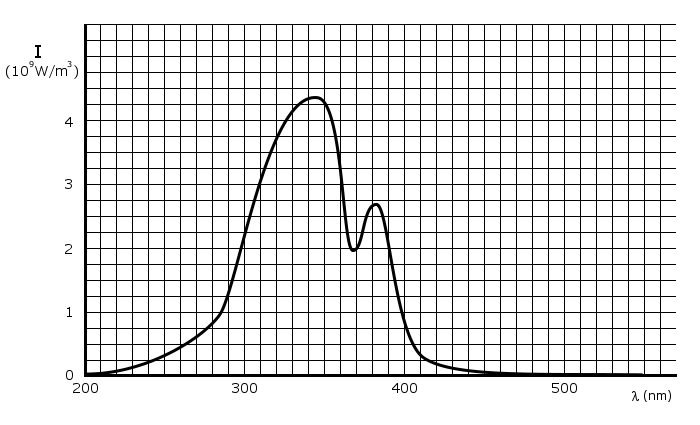
\includegraphics[width=0.49\textwidth]{2011-lahg-04-I}
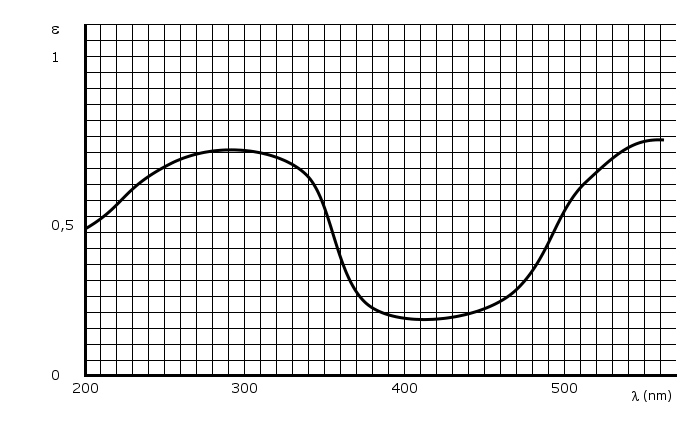
\includegraphics[width=0.49\textwidth]{2011-lahg-04-epsilon}
\end{center}
\fi


\ifHint
Kuna kogu Smurfile langenud valgusest $I$ neeldub Smurfil vaid $ I \cdot\varepsilon $, kujutab $ I \cdot \varepsilon $ graafik Smurfil neeldunud valguse intensiivsust lainepikkuse kohta sõltuvalt lainepikkusest. Graafiku alune pindala annabki Smurfil neeldunud soojushulga. 
\fi


\ifSolution
Kuna kogu Smurfile langenud valgusest $I$ neeldub Smurfil vaid $ I \cdot
\varepsilon $, kujutab $ I \cdot \varepsilon $ graafik Smurfil neeldunud valguse
intensiivsust lainepikkuse kohta sõltuvalt lainepikkusest. Konstrueerime
nimetatud graafiku. Selleks loeme jooniselt erinevate $ \lambda $ väärtustele
vastavad $ I $ ja $ \varepsilon $ väärtused ning arvutame nende korrutised, vt
tabelit. Tabeli põhjal konstrueeritud joonise ning loeme graafiku alla jäänud
pindala, mis on võrdne Smurfil neeldunud valguse intensiivsusega
\[
I_{\mathrm{kokku}} =
(162+\frac{74}{2}) \cdot \SI{1}{\frac{W}{m^2}} = \SI{199}{\frac{W}{m^2}}.
\]
Kuna kiirguse intensiivsus näitab võimsust pindalaühiku kohta, saab Smurf kokku soojushulga
\[ Q = I_{\mathrm{kokku}}St =
\SI{199}{\frac{W}{m^2}} \cdot \SI{0,1}{m^2} \cdot \SI{10}{min} \cdot
\SI{60}{\frac{s}{min}} \approx \SI{12}{kJ}.\]


\begin{tabular}{r|c|c|c|c|c|c|c|c|c|c|c|c|c|c|c|c|c|}
	\hline
	$ \lambda \ ($nm$) $&$ 200 $&$ 220 $&$ 240 $&$ 260 $&$ 280 $&$ 300 $&$ 320 $&$ 340 $&$ 350 $\\
	\hline
	$ I \ (10^9 \cdot \frac{\text{W}}{\text{m}^3}) $&$ 0,00 $&$ 0,05 $&$ 0,24 $&$ 0,45 $&$ 0,85 $&$ 2,25 $&$ 3,75 $&$ 4,35 $&$ 4,25 $\\
	\hline
	$ \varepsilon $&$ 0,46 $&$ 0,54 $&$ 0,62 $&$ 0,68 $&$ 0,70 $&$ 0,70 $&$ 0,68 $&$ 0,62 $&$ 0,53 $\\
	\hline
	$ I \cdot \varepsilon \ (10^9 \cdot \frac{\text{W}}{\text{m}^3}) $&$ 0,00 $&$ 0,03 $&$ 0,15 $&$ 0,31 $&$ 0,60 $&$ 1,58 $&$ 2,55 $&$ 2,70 $&$ 2,25 $\\
	\hline
	\hline
	$ \lambda \ ($nm$) $&$ 360 $&$ 370 $&$ 380 $&$ 400 $&$ 420 $&$ 440 $&$ 460 $&$ 480 $\\
	\hline
	$ I \ (10^9 \cdot \frac{\text{W}}{\text{m}^3}) $&$ 3,25 $&$ 2,00 $&$ 2,70 $&$ 0,85 $&$ 0,20 $&$ 0,10 $&$ 0,05 $&$ 0,00 $\\
	\hline
	$ \varepsilon $&$ 0,37 $&$ 0,25 $&$ 0,22 $&$ 0,18 $&$ 0,18 $&$ 0,20 $&$ 0,23 $&$ 0,33 $\\
	\hline
	$ I \cdot \varepsilon \ (10^9 \cdot \frac{\text{W}}{\text{m}^3}) $&$ 1,20 $&$ 0,50 $&$ 0,59 $&$ 0,15 $&$ 0,04 $&$ 0,02 $&$ 0,01 $&$ 0,00 $\\ 	
\end{tabular}

\begin{center}
	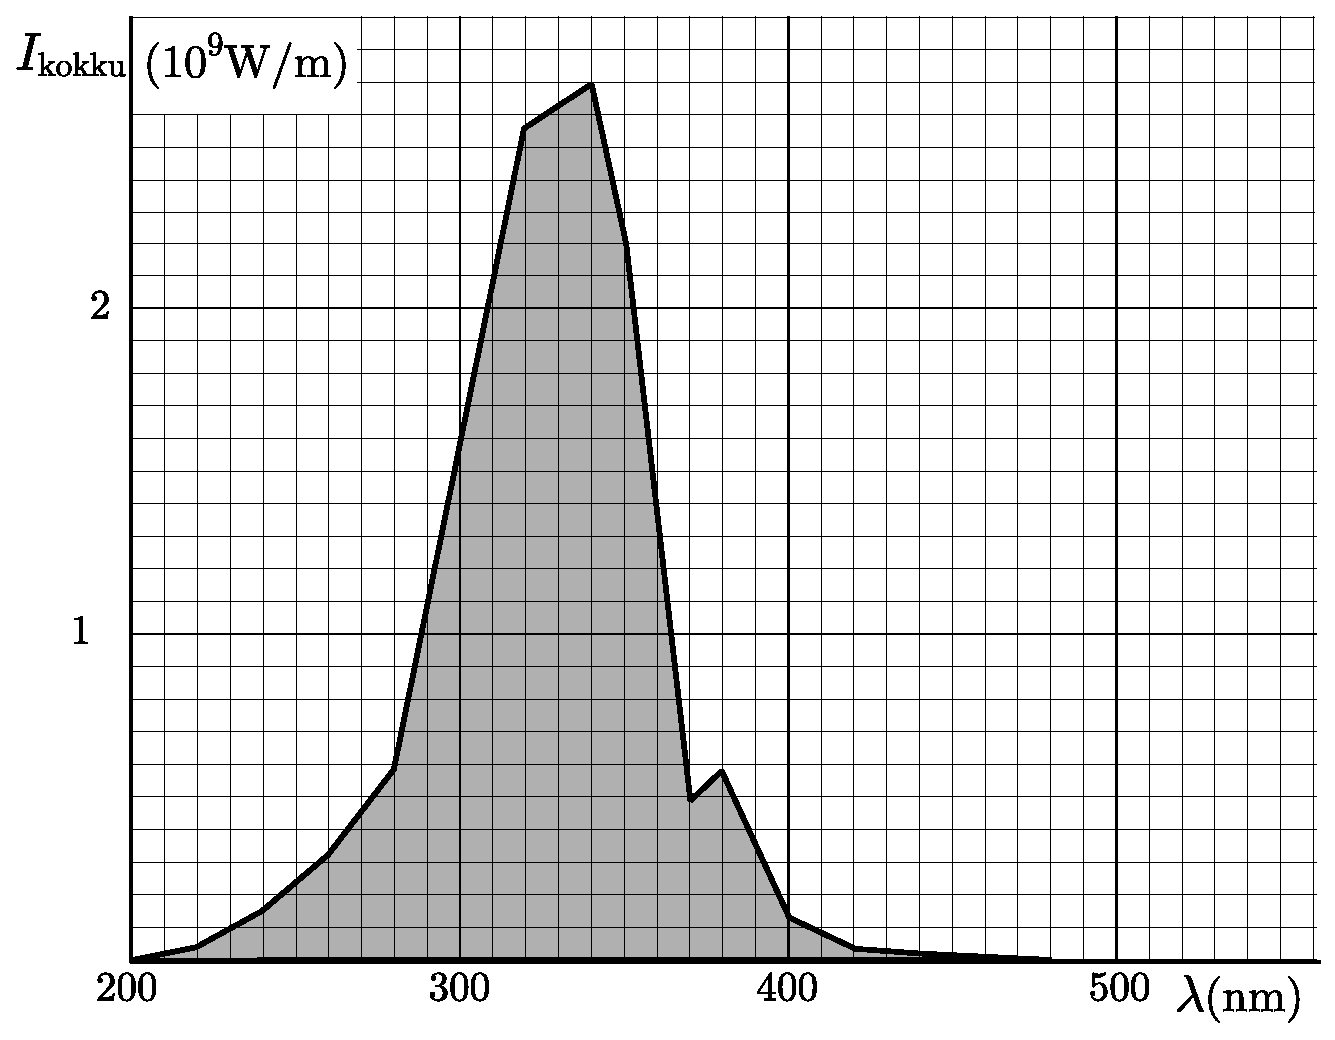
\includegraphics[width=80mm]{2011-lahg-04-intensity}
\end{center}
\fi


\ifEngStatement
% Problem name: Smurf in solarium
Smurf spent $t = \SI{10}{min} $ under the lights of a solarium. What heat $ Q $ did Smurf receive? The incident light spectrum $I$ of Smurf (intensity per wavelength depending on the wavelength of the light, unit \SI{10e9}{W/m^3}) and the absorbed spectrum $\varepsilon$ of Smurf (the relation between the absorbed and incident intensity as a function of wavelength) are given in the figure. The effective area where the light falls on Smurf is $ S = \SI{0,1}{m^2} $.

\begin{center}
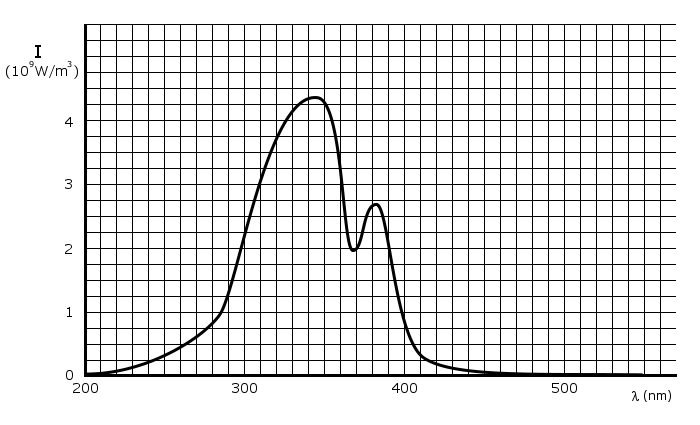
\includegraphics[width=0.49\textwidth]{2011-lahg-04-I}
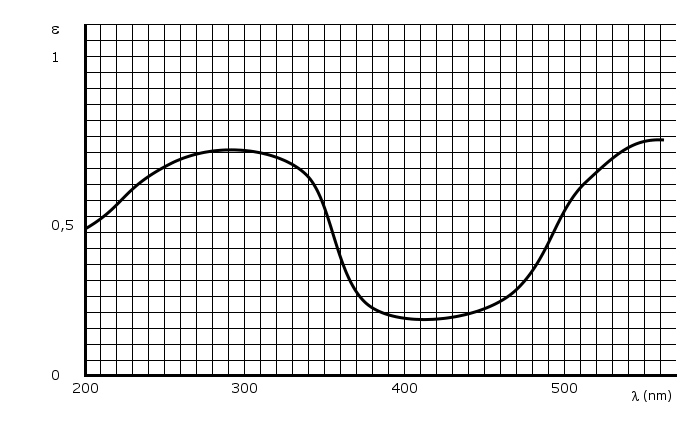
\includegraphics[width=0.49\textwidth]{2011-lahg-04-epsilon}
\end{center}
\fi


\ifEngHint
Because from all of the light $I$ that falls on Smurf only $ I \cdot\varepsilon $ is absorbed by him, the $ I \cdot \varepsilon $ graph depicts the intensity of light absorbed on Smurf per wavelength depending on wavelength. The area below the graph gives the heat absorbed by Smurf.
\fi


\ifEngSolution
Because from all of the light $I$ that falls on the Smurf only $ I \cdot \varepsilon $ is absorbed by the Smurf then the $ I \cdot \varepsilon $ graph depicts the intensity of the light absorbed by the Smurf per wavelength depending on the wavelength. Let us construct the mentioned graph. For this we need to read the values of $I$ and $ \varepsilon $ corresponding to different values of $ \lambda $ and calculate their products (see table). We construct a figure based on the table and read the area that stays under the graph which is equal to the intensity of the light absorbed by the Smurf $I_{\mathrm{total}} =
(162+\frac{74}{2}) \cdot \SI{1}{\frac{W}{m^2}} = \SI{199}{\frac{W}{m^2}}$. Because the intensity of radiation is also the power per unit of area then the Smurf gets a total amount of heat
\[ Q = I_{\mathrm{total}}St =
\SI{199}{\frac{W}{m^2}} \cdot \SI{0,1}{m^2} \cdot \SI{10}{min} \cdot
\SI{60}{\frac{s}{min}} \approx \SI{12}{kJ}.\]


\begin{tabular}{r|c|c|c|c|c|c|c|c|c|c|c|c|c|c|c|c|c|}
	\hline
	$ \lambda \ ($nm$)                                               $&$ 200  $&$ 220  $&$ 240  $&$ 260  $&$ 280  $&$ 300  $&$ 320  $&$ 340  $&$ 350  $\\
	\hline
	$ I \ (10^9 \cdot \frac{\text{W}}{\text{m}^3})                   $&$ 0,00 $&$ 0,05 $&$ 0,24 $&$ 0,45 $&$ 0,85 $&$ 2,25 $&$ 3,75 $&$ 4,35 $&$ 4,25 $\\
	\hline
	$ \varepsilon                                                    $&$ 0,46 $&$ 0,54 $&$ 0,62 $&$ 0,68 $&$ 0,70 $&$ 0,70 $&$ 0,68 $&$ 0,62 $&$ 0,53 $\\
	\hline
	$ I \cdot \varepsilon \ (10^9 \cdot \frac{\text{W}}{\text{m}^3}) $&$ 0,00 $&$ 0,03 $&$ 0,15 $&$ 0,31 $&$ 0,60 $&$ 1,58 $&$ 2,55 $&$ 2,70 $&$ 2,25 $\\
	\hline
	\hline
	$ \lambda \ ($nm$)                                               $&$ 360  $&$ 370  $&$ 380  $&$ 400  $&$ 420  $&$ 440  $&$ 460  $&$ 480  $\\
	\hline
	$ I \ (10^9 \cdot \frac{\text{W}}{\text{m}^3})                   $&$ 3,25 $&$ 2,00 $&$ 2,70 $&$ 0,85 $&$ 0,20 $&$ 0,10 $&$ 0,05 $&$ 0,00 $\\
	\hline
	$ \varepsilon                                                    $&$ 0,37 $&$ 0,25 $&$ 0,22 $&$ 0,18 $&$ 0,18 $&$ 0,20 $&$ 0,23 $&$ 0,33 $\\
	\hline
	$ I \cdot \varepsilon \ (10^9 \cdot \frac{\text{W}}{\text{m}^3}) $&$ 1,20 $&$ 0,50 $&$ 0,59 $&$ 0,15 $&$ 0,04 $&$ 0,02 $&$ 0,01 $&$ 0,00 $\\ 	
\end{tabular}

\begin{center}
	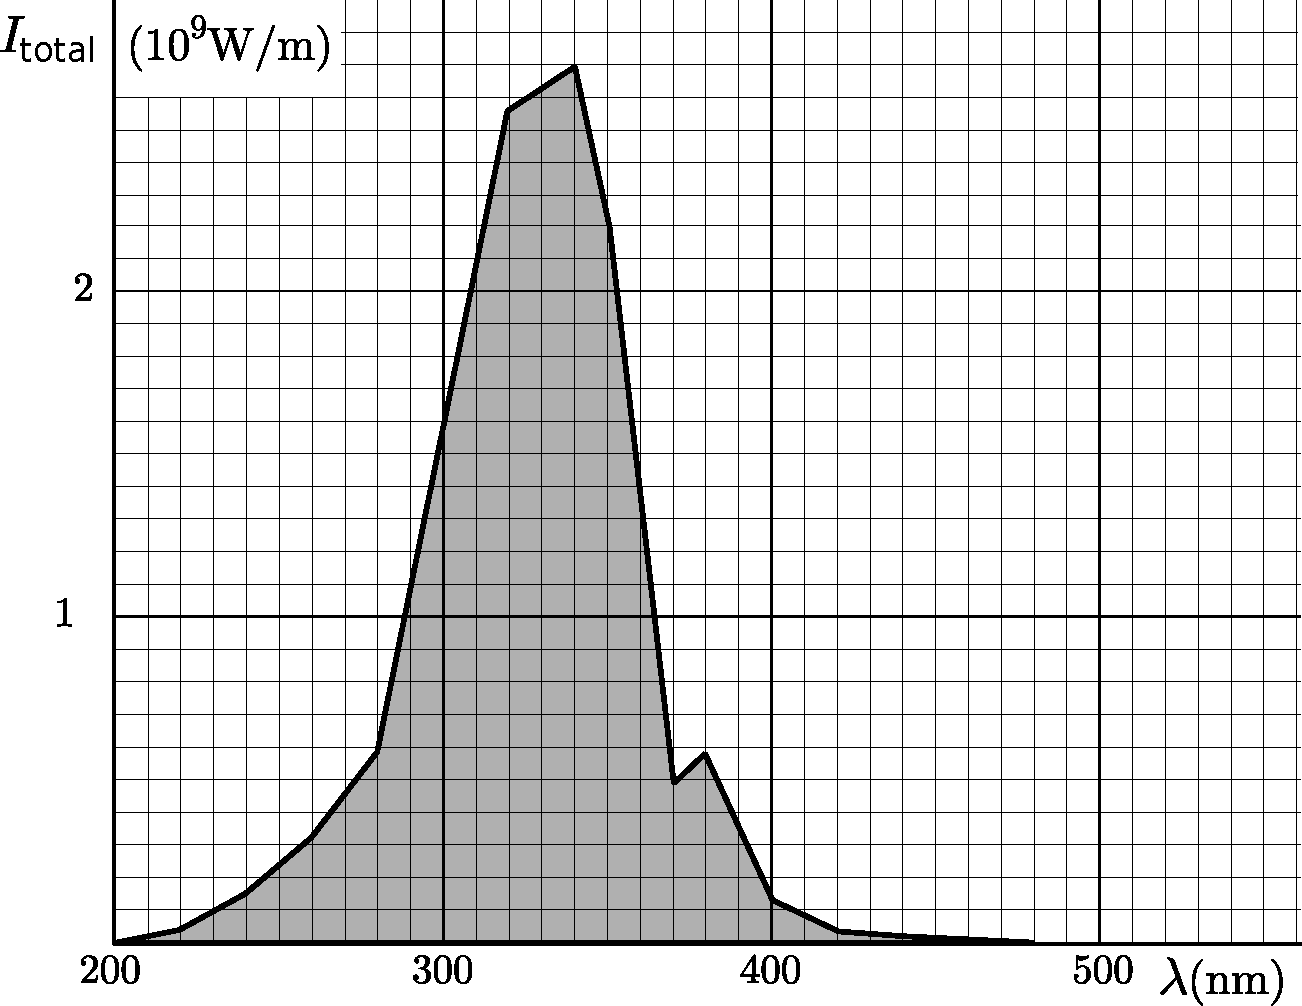
\includegraphics[width=80mm]{2011-lahg-04-intensity-ing}
\end{center}
\fi
}